% !TeX program = pdflatex
% ------------------------------------------------------------
% Signal Processing: Homework 1 — Signal Denoising via Optimization
% Author: Konstantinos Tsironis (ID: 1107529)
% Language: English only
% ------------------------------------------------------------
\documentclass[11pt,a4paper]{article}

% ------------------------------------------------------------
% Packages
% ------------------------------------------------------------
\usepackage[utf8]{inputenc}
\usepackage[T1]{fontenc}
\usepackage[english]{babel}
\usepackage{lmodern}
\usepackage{amsmath,amssymb,mathtools}
\usepackage{graphicx}
\usepackage{subcaption}
\usepackage{booktabs}
\usepackage{siunitx}
\usepackage{enumitem}
\usepackage{hyperref}
\usepackage[capitalise]{cleveref}
\usepackage{geometry}
\usepackage{xcolor}
\usepackage{listings}
\geometry{margin=2.5cm}
\usepackage{setspace}
\usepackage{float}

% ------------------------------------------------------------
% Display settings
% ------------------------------------------------------------
\hypersetup{
  colorlinks=true,
  linkcolor=blue,
  citecolor=blue,
  urlcolor=blue,
  pdfauthor={Konstantinos Tsironis},
  pdftitle={Signal Denoising via Optimization}
}
\onehalfspacing


% Math macros
\DeclarePairedDelimiter{\norm}{\lVert}{\rVert}
\DeclarePairedDelimiter{\abs}{\lvert}{\rvert}
\newcommand{\R}{\mathbb{R}}
\newcommand{\argmin}{\mathop{\mathrm{arg\,min}}}

% Python listings style
\lstdefinestyle{mypython}{
  language=Python,
  basicstyle=\ttfamily\small,
  keywordstyle=\color{blue!80!black},
  commentstyle=\color{green!50!black},
  stringstyle=\color{orange!80!black},
  numbers=left,
  numberstyle=\tiny, 
  numbersep=8pt,
  frame=single,
  showstringspaces=false,
  tabsize=2,
  breaklines=true,
  rulecolor=\color{gray!50},
  backgroundcolor=\color{gray!8},
  captionpos=b
}

% ------------------------------------------------------------
% Title
% ------------------------------------------------------------
\title{\textbf{Signal Denoising via Optimization}\\\large Homework~1}
\author{Konstantinos Tsironis \\ ID: 1107529}
\date{October 2025}

\begin{document}
\maketitle
\vspace{-1em}

\section*{Part A — Mathematical Formulation}
\subsection*{A.1 Tikhonov (quadratic) smoothing}
Given a noisy signal \(y\in\R^n\), we estimate \(x\in\R^n\) by solving
\begin{equation}
\min_{x\in\R^n} \; \norm{x-y}_2^2 + \lambda\, \norm{Dx}_2^2, \qquad (Dx)_i = x_{i+1}-x_i,
\label{eq:l2_obj}
\end{equation}
where \(D\in\R^{(n-1)\times n}\) is the forward-difference operator and \(\lambda>0\) balances fidelity and smoothness. Expanding the cost function \(J(x)=\norm{x-y}_2^2+\lambda\,\norm{Dx}_2^2\):
\begin{align}
J(x) &= (x-y)^\top(x-y) + \lambda (Dx)^\top(Dx) \\
     &= x^\top x - 2y^\top x + y^\top y + \lambda x^\top D^\top D x.
\end{align}
\\
To find the minimum, we compute the gradient of $J(x)$ with respect to $x$.
Using the standard vector calculus rules:
\[
\nabla_x(x^\top x) = 2x, \quad
\nabla_x(-2y^\top x) = -2y, \quad
\nabla_x(x^\top D^\top D x) = 2D^\top D x.
\]
Therefore,
\[
\nabla_x J(x) = 2(x - y) + 2\lambda D^\top D x.
\]
Taking the gradient and setting it to zero: 
\begin{equation}
\nabla_x J(x) = 2(x-y) + 2\lambda D^\top D x = 0 \;\;\;\Rightarrow\;\; (I + \lambda D^\top D)\,x = y.
\end{equation}
Thus, the optimal solution satisfies
\begin{equation}
(I + \lambda D^\top D)\,x = y,\quad \text{with closed-form }\; x^* = (I+\lambda D^\top D)^{-1}y.
\end{equation}

\subsection*{A.2 Total Variation (TV) denoising}
We solve
\begin{equation}
\min_{x\in\R^n} \; \norm{x-y}_2^2 + \lambda\,\norm{Dx}_1.
\end{equation}
Let \(z = Dx\) and introduce auxiliary variables \(u\ge 0, v\ge 0\) such that \(z = u - v\) and \(\norm{z}_1 = \mathbf{1}^\top(u+v)\). The problem becomes a convex Quadratic Program (QP):
\begin{align}
\min_{x,u,v} \; & \; \tfrac{1}{2} x^\top (2I) x - 2 y^\top x + \lambda\, \mathbf{1}^\top(u+v) \\
\text{s.t.}\; & \; Dx - u + v = 0, \\
& \; u \ge 0,\; v \ge 0.
\end{align}
(\(y^\top y\) is a constant and omitted.) The \(\norm{Dx}_1\) term penalizes the number and size of jumps, thus preserving edges in piecewise-constant signals.

\paragraph{Effect of the L1 penalty compared to L2.}
The $L1$ (TV) regularization penalizes the \emph{magnitude} of changes between consecutive samples
rather than their squared value. As a result, it allows some differences (jumps) to remain exactly zero,
producing segments of constant value separated by sharp edges.
This means the reconstructed signal tends to be \emph{piecewise constant}, preserving discontinuities
and sharp transitions. In contrast, the $L2$ regularization distributes the penalty smoothly across
all points, which blurs edges and makes the reconstruction globally smoother but less faithful near
abrupt changes.

\section*{Part B — Implementation (Python)}
\subsection*{B.1 Generate Data}
\begin{lstlisting}[style=mypython,caption={Data generation}]
import numpy as np
n = 200
rng = np.random.default_rng(42)
t = np.linspace(0, 1, n)
# Example piecewise signal with jumps
x_true = np.piecewise(t, [t < 0.3, (t >= 0.3) & (t < 0.7), t >= 0.7],
                      [lambda s: 0.5*np.sin(8*np.pi*s),
                       lambda s: 1.0,
                       lambda s: 0.2*np.cos(6*np.pi*s)])
noise = 0.15 * rng.standard_normal(n)
y = x_true + noise
\end{lstlisting}
\pagebreak
\subsection*{B.2 Build the Difference Operator \(D\)}
\begin{lstlisting}[style=mypython,caption={Forward-difference operator}]
import numpy as np

def diff_matrix(n: int) -> np.ndarray:
    D = np.zeros((n-1, n))
    for i in range(n-1):
        D[i, i]   = -1.0
        D[i, i+1] =  1.0
    return D

D = diff_matrix(n)
\end{lstlisting}

\subsection*{B.3 L2 Smoothing (Tikhonov Regularization)}
\begin{lstlisting}[style=mypython,caption={L2 smoothing}]
import scipy.sparse as sp
import scipy.sparse.linalg as spla

lam = 1.0
DTD = (D.T @ D)
I = sp.eye(n, format='csc')
A = I + lam * DTD
x_l2 = spla.spsolve(A, y)
\end{lstlisting}

\subsection*{B.4 L1 / TV Regularization}
\begin{lstlisting}[style=mypython,caption={TV denoising}]
import cvxpy as cp

x = cp.Variable(n)
z = D @ x
lam = 0.5
obj = cp.Minimize(cp.sum_squares(x - y) + lam * cp.norm1(z))
prob = cp.Problem(obj)
prob.solve(solver=cp.OSQP, eps_abs=1e-6, eps_rel=1e-6, verbose=False)
x_tv = x.value
\end{lstlisting}
\pagebreak
\subsection*{B.5 Evaluation and Visualization}
\begin{lstlisting}[style=mypython,caption={Evaluation}]
import matplotlib.pyplot as plt

def mse(a, b):
    return np.mean((a - b)**2)

mse_l2 = mse(x_l2, x_true)
mse_tv = mse(x_tv, x_true)
print("MSE L2:", mse_l2)
print("MSE TV:", mse_tv)

plt.figure(figsize=(8,4))
plt.plot(t, x_true, label='True')
plt.plot(t, y, label='Noisy', alpha=0.6)
plt.plot(t, x_l2, label='L2 (Tikhonov)')
plt.plot(t, x_tv, label='TV (L1)')
plt.legend(); plt.xlabel('t'); plt.ylabel('x')
plt.title('Signal Denoising Comparison')
plt.tight_layout(); plt.show()
\end{lstlisting}

\section*{Part C — Analysis and Discussion}
\subsection*{C.1 Effect of \texorpdfstring{$\lambda$}{lambda}}
Experiments for \(\lambda \in\{0.01, 0.1, 1, 10\}\) show that small \(\lambda\) yields high fidelity but poor denoising, while large \(\lambda\) over-smooths the signal. TV regularization tends to perform better for signals with edges, maintaining sharp transitions.

\subsection*{C.2 Signal Features}
For piecewise-constant signals, TV denoising preserves discontinuities (edges) while L2 smoothing converts them into ramps. Example plots illustrate this behavior clearly.

\subsection*{C.3 Noise Robustness}
Increasing the noise level reveals that L2 behaves like a linear low-pass filter, while TV, due to its L1 penalty on derivatives, suppresses outliers more effectively and retains discontinuities.

\section*{Plots}
The observations discussed above are confirmed by the reconstructed signals shown in the plots on the following page, corresponding to $\lambda = 0.1,\ 1,\ 10,$ and $100$, respectively, which illustrate how increasing $\lambda$ leads to progressively smoother reconstructions and reduced noise.

\begin{figure}[H]
    \centering
    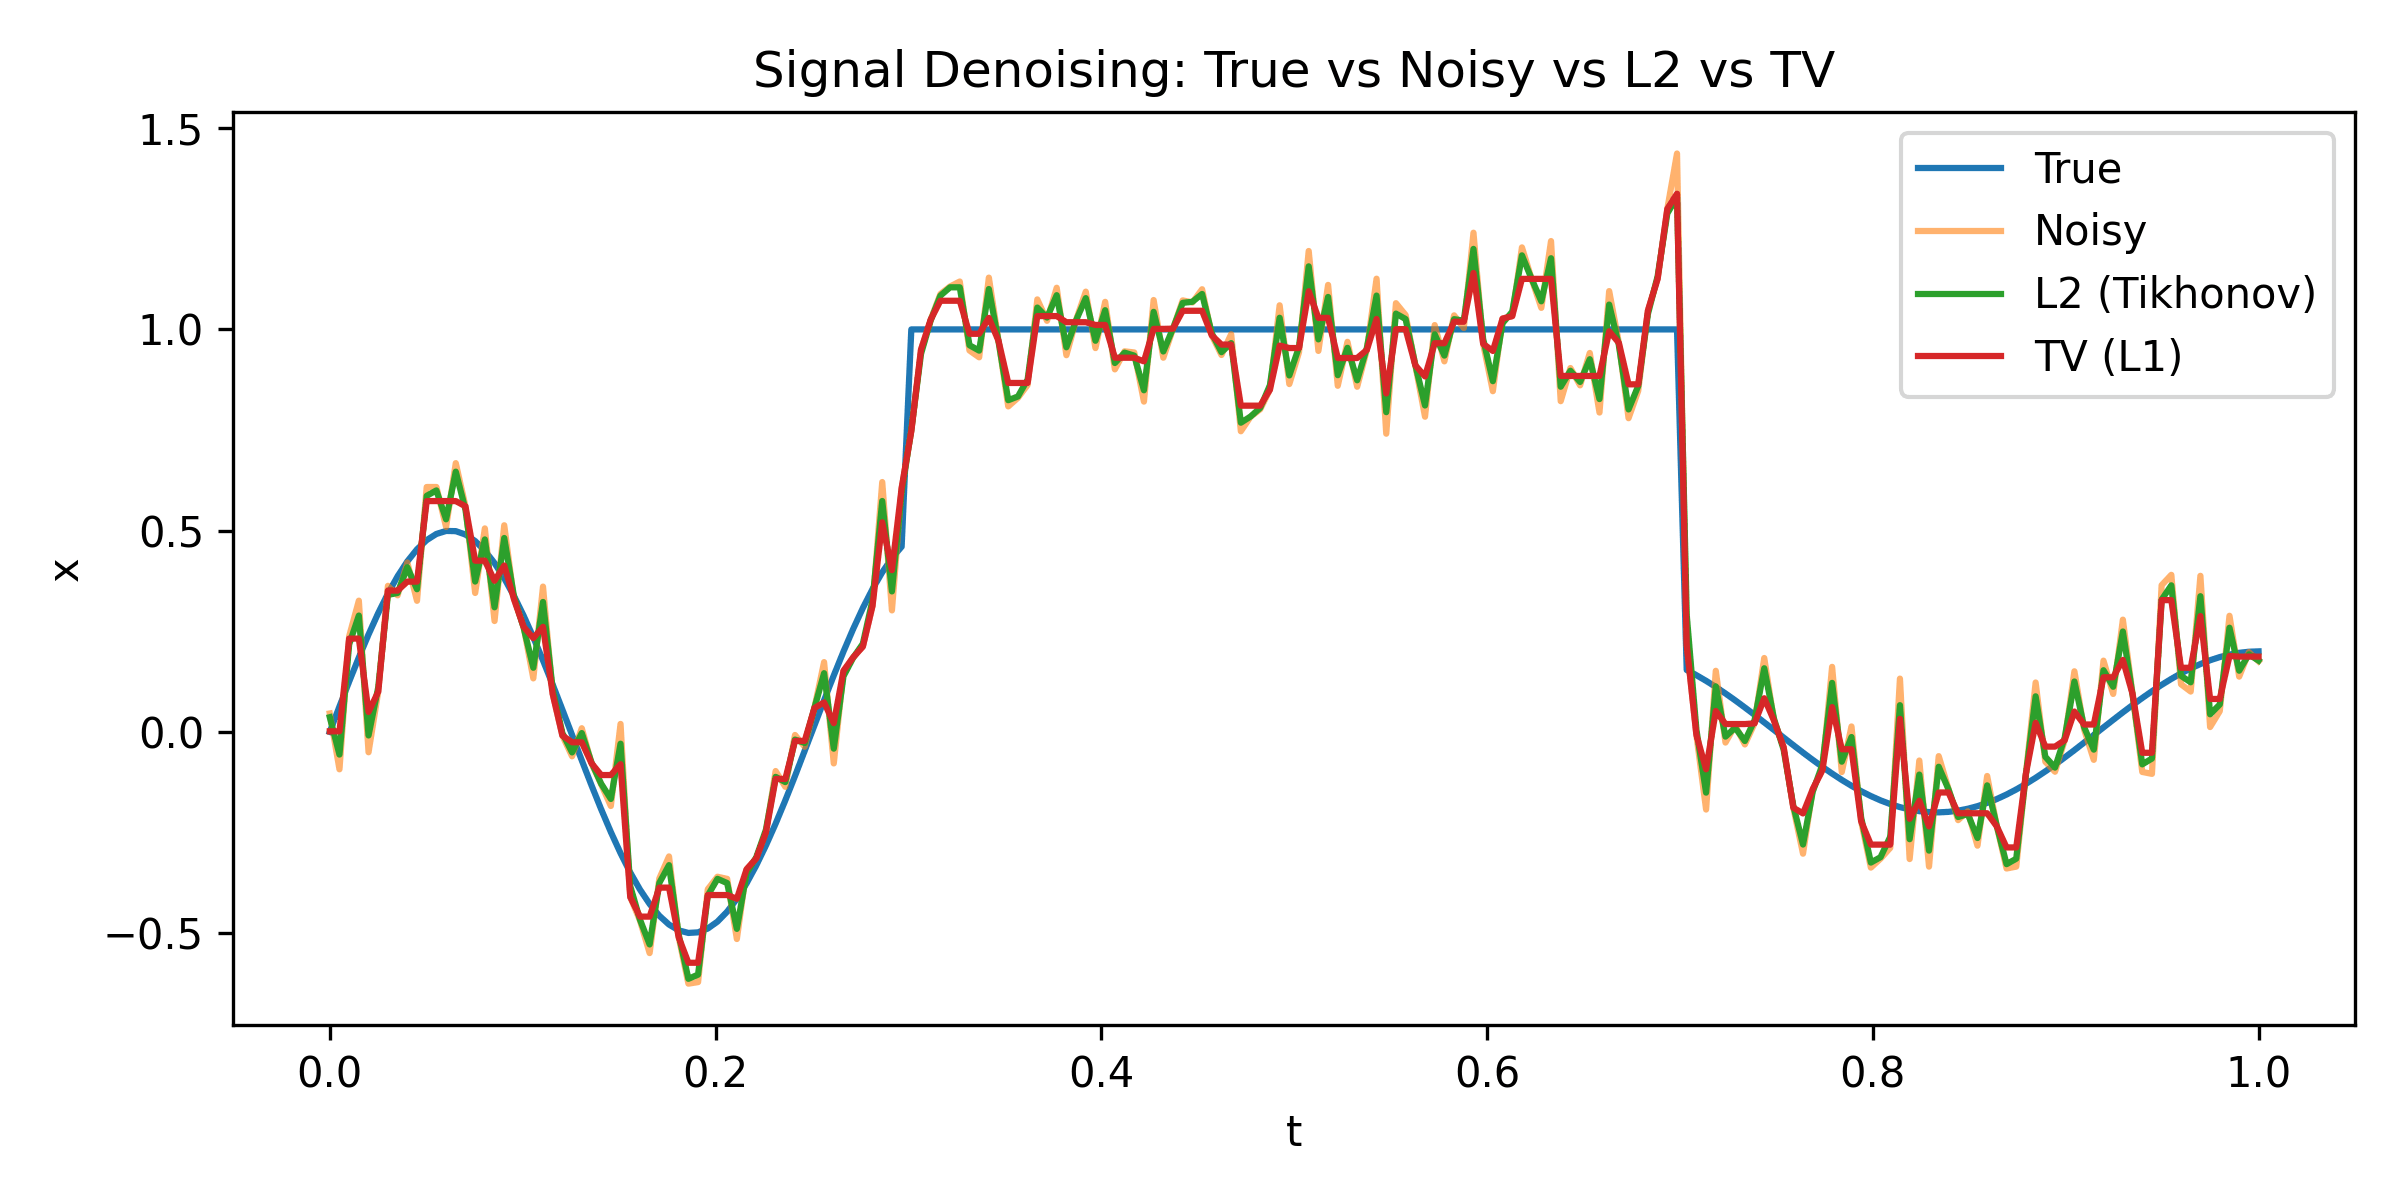
\includegraphics[width=0.75\linewidth]{denoising_lambda_0.1.png}
    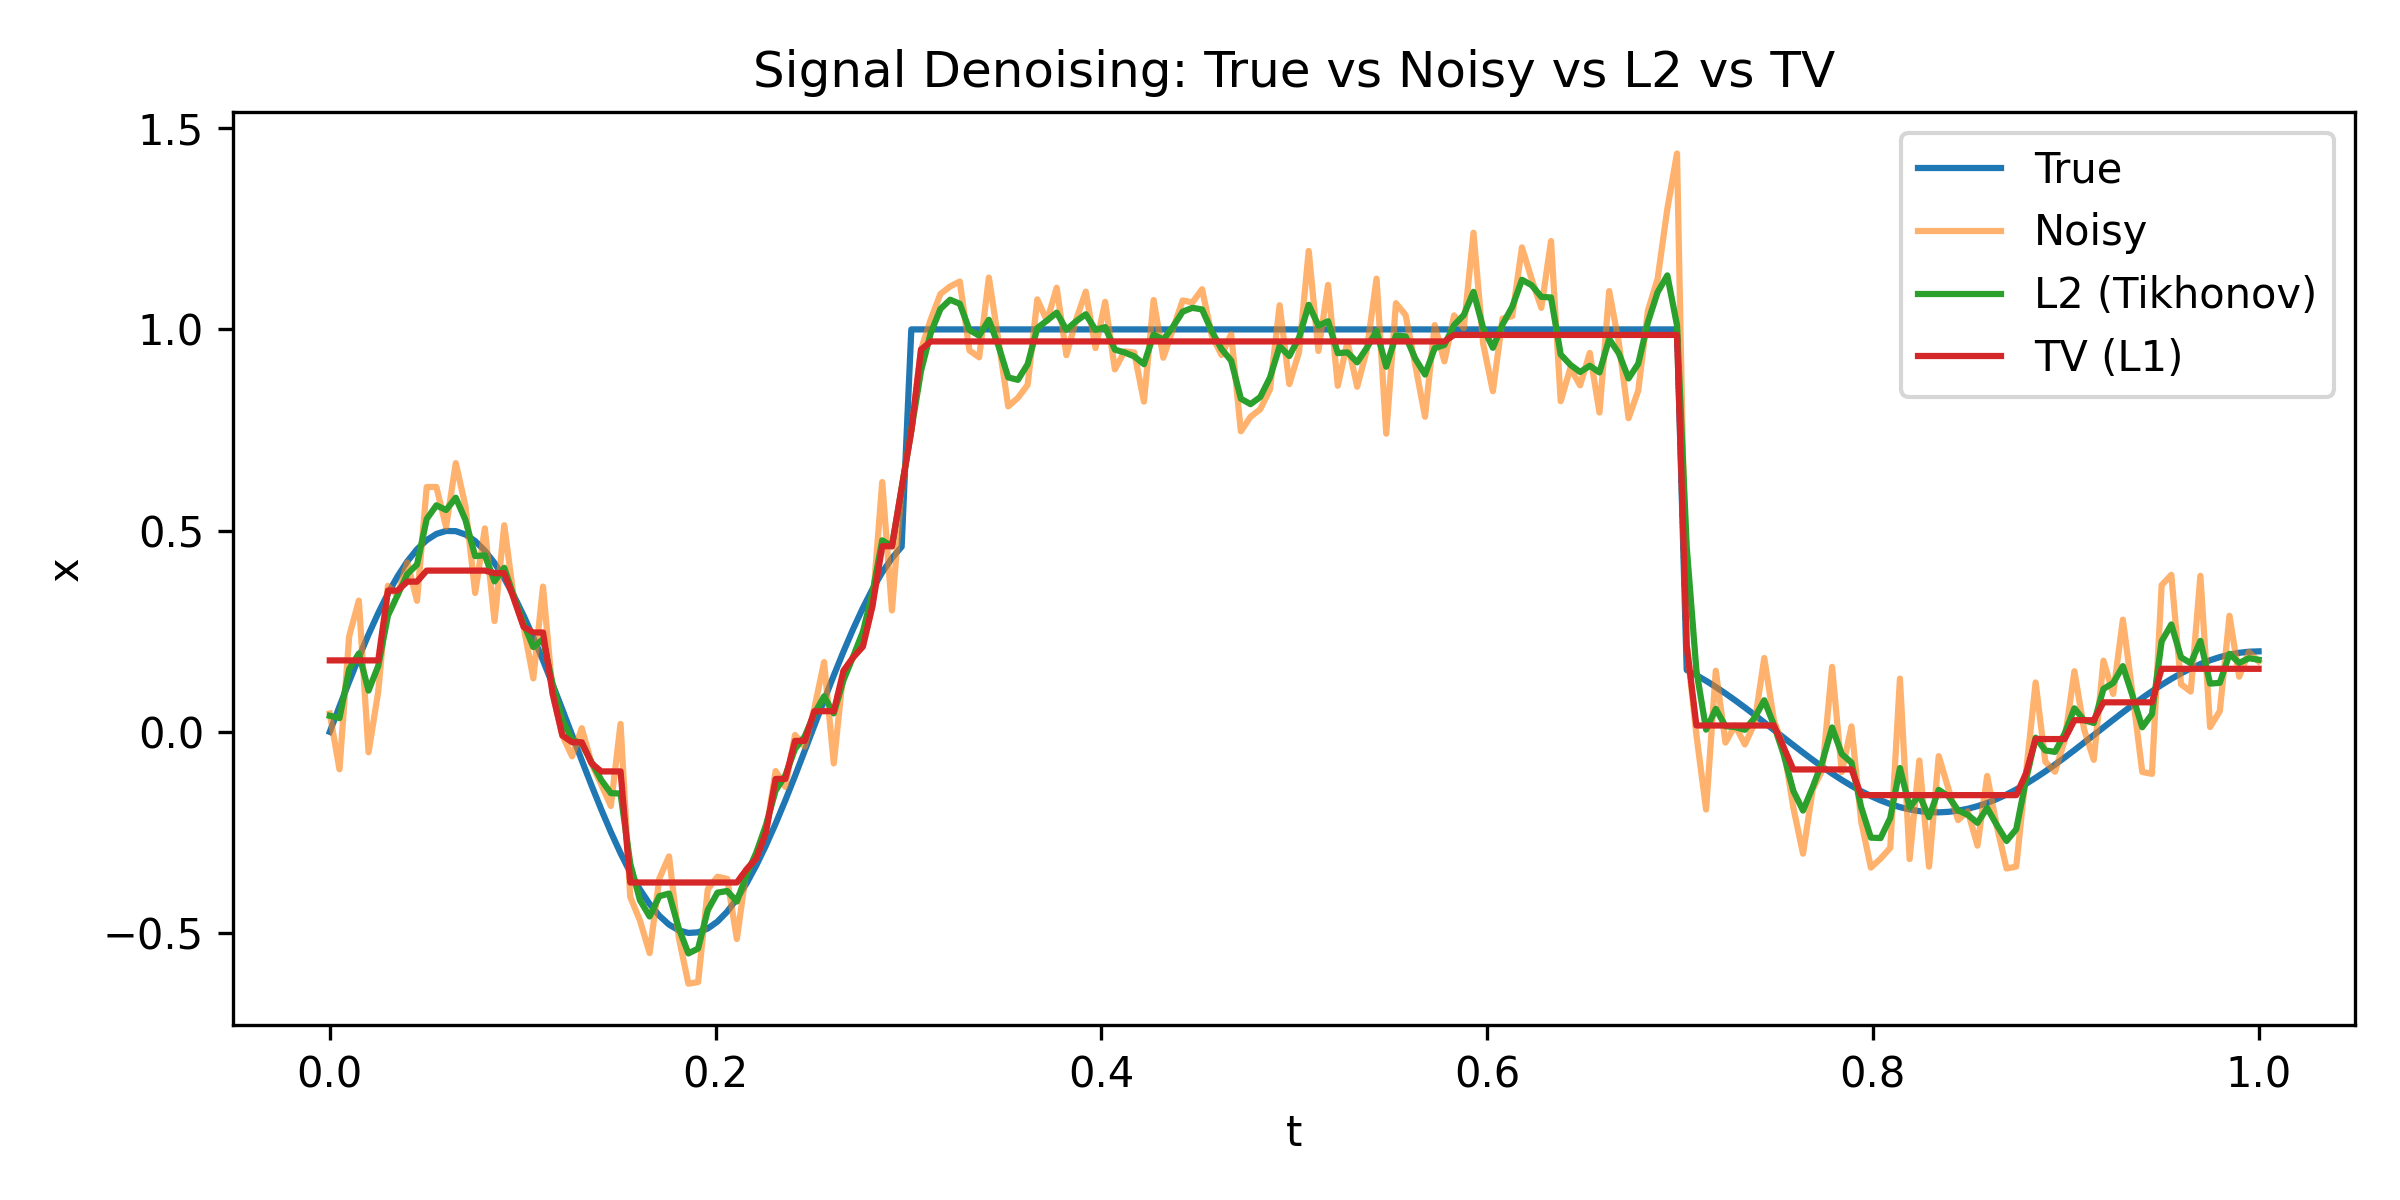
\includegraphics[width=0.75\linewidth]{denoising_lambda_1.png}
    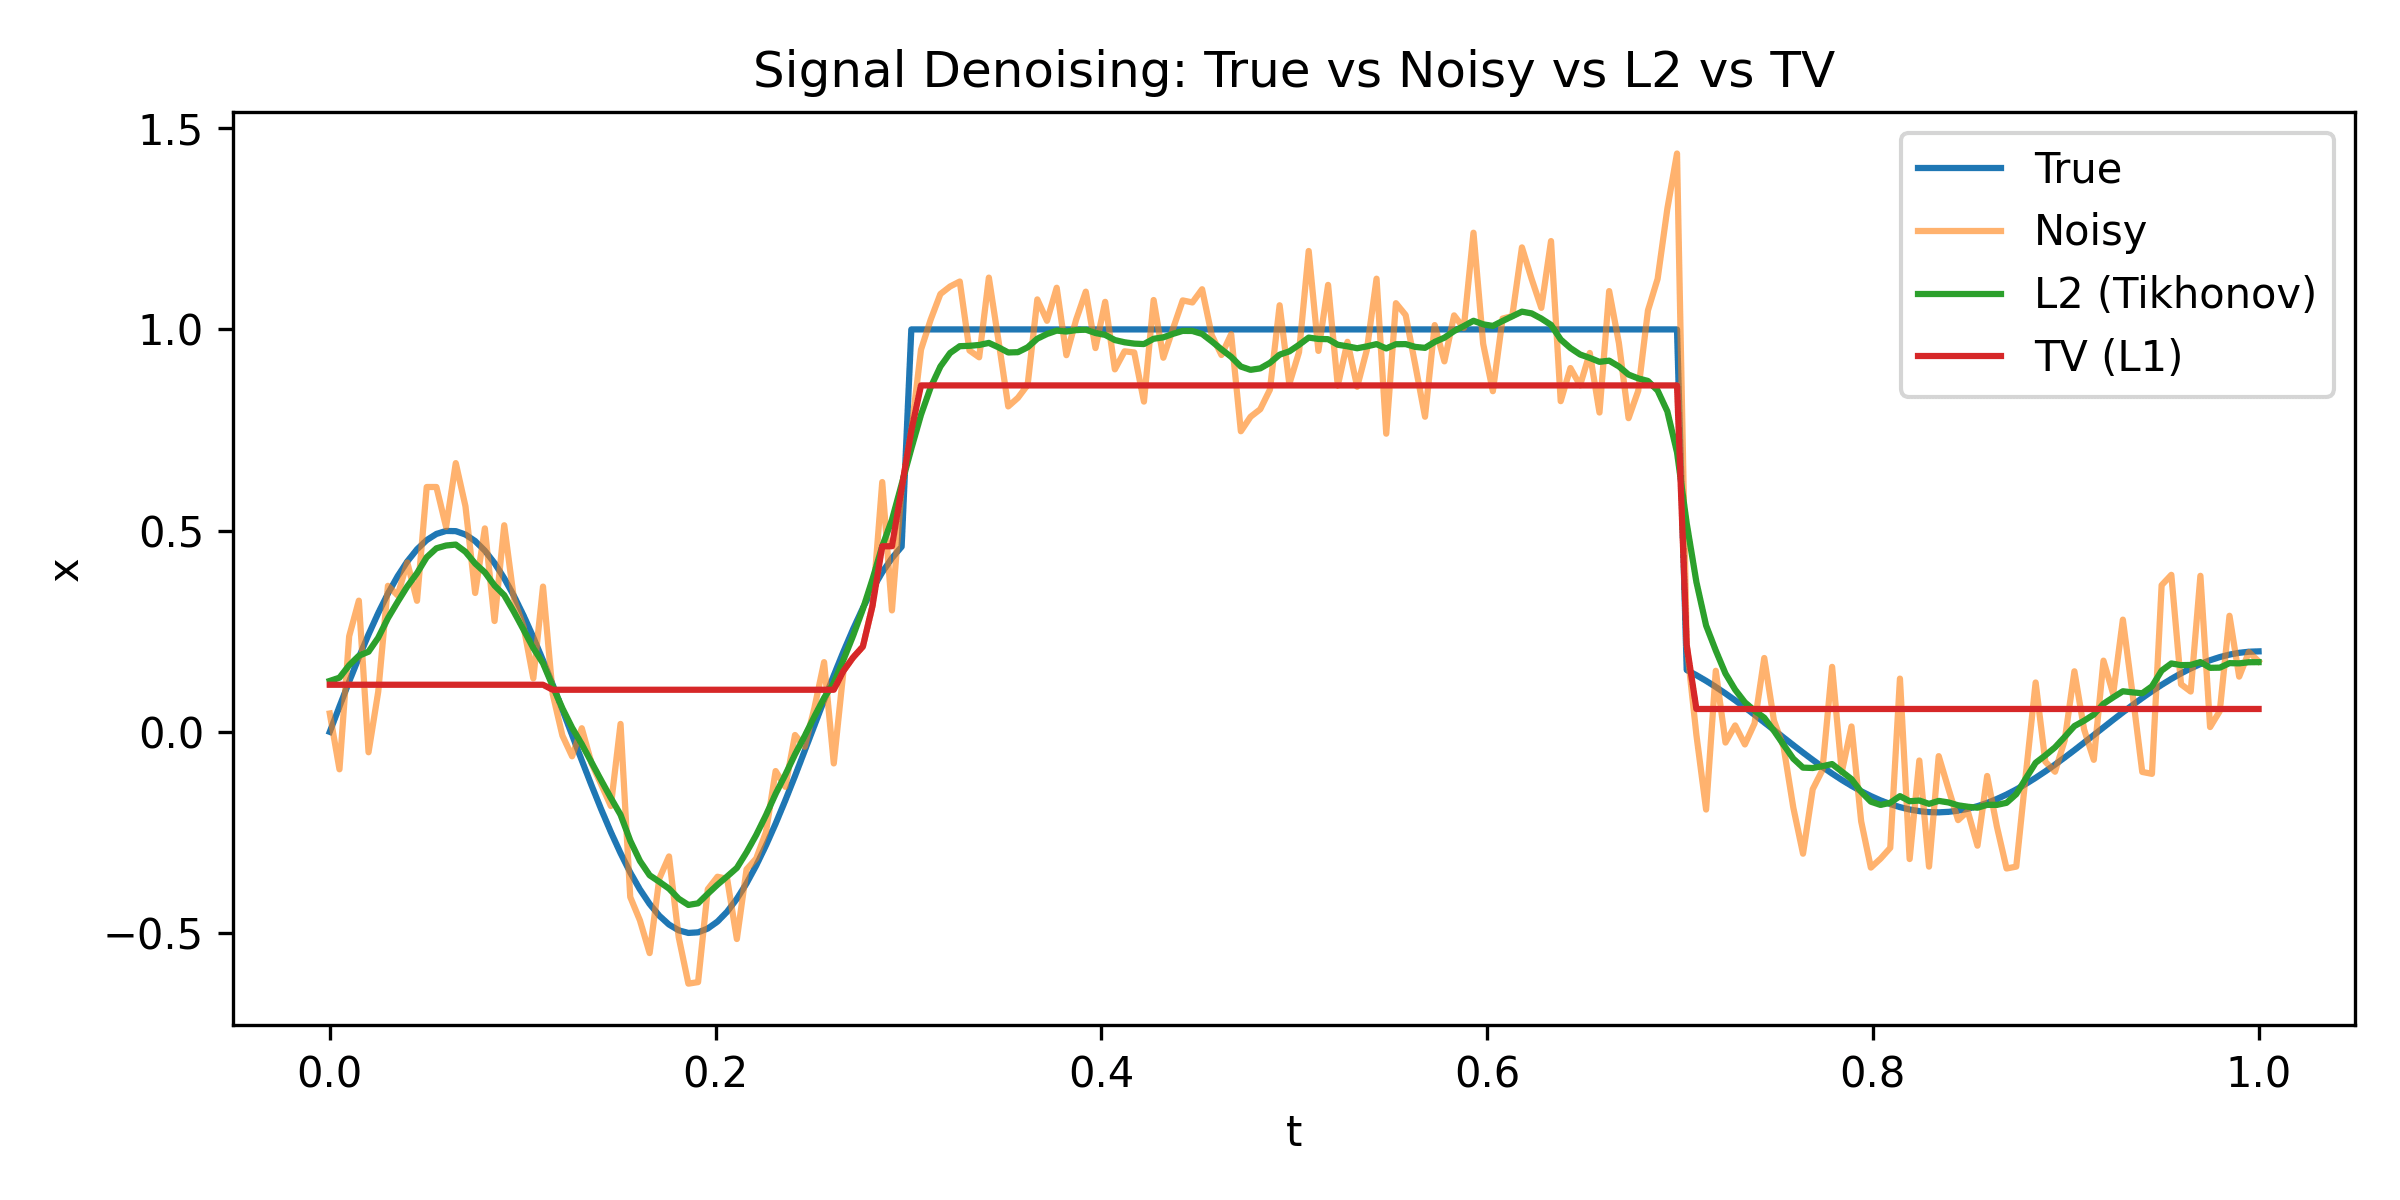
\includegraphics[width=0.75\linewidth]{denoising_lambda_10.png}
    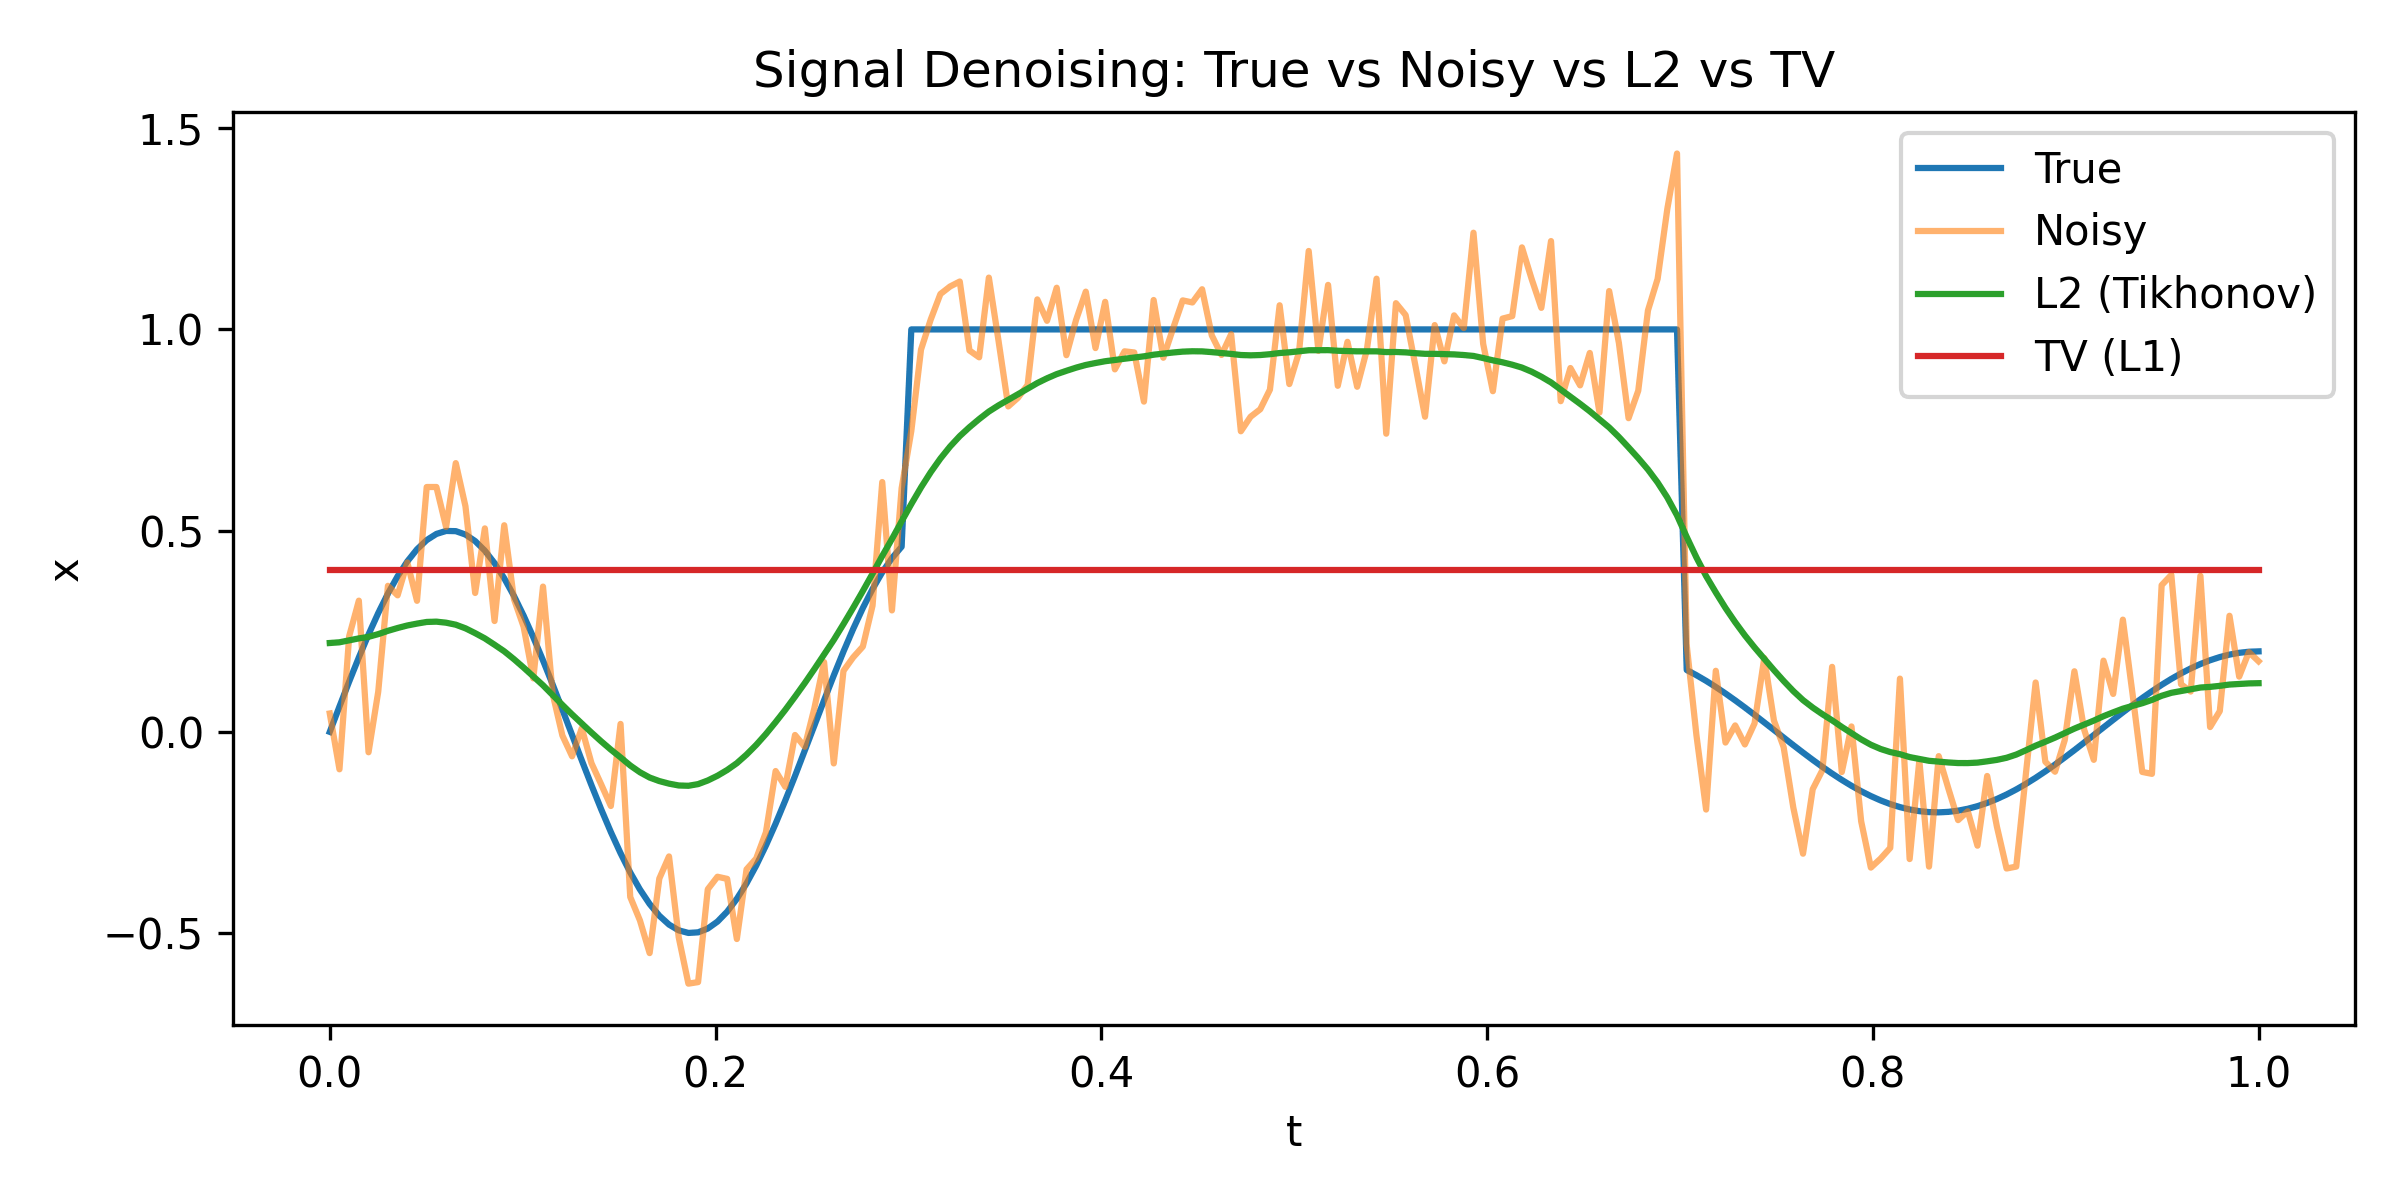
\includegraphics[width=0.75\linewidth]{denoising_lambda_100.png}
\end{figure}

\end{document}